% chktex-file 44
\documentclass[a4paper,12pt]{article}

% Paquetes básicos
\usepackage[utf8]{inputenc}
\usepackage[T1]{fontenc}
\usepackage[spanish]{babel}
\usepackage{graphicx}
\usepackage{xcolor}
\usepackage{lipsum}
\usepackage{geometry}
\usepackage{eurosym}
\geometry{top=3cm, bottom=3cm, left=2.5cm, right=2.5cm}

% Paquetes para diseño
\usepackage{titlesec}
\usepackage{fancyhdr}
\usepackage{amsmath}
\usepackage{amssymb}
\usepackage{hyperref}

% Paquetes para el entorno lstlisting
\usepackage{listings}
\usepackage{inconsolata}

%encabezado y pie de página nivel profesional
\usepackage{fancyhdr}
\pagestyle{fancy}
\fancyhf{}
\fancyhead[L]{\leftmark}
\fancyhead[R]{\rightmark}
\fancyfoot[L]{\textbf{Ismael Sallami Moreno - GIIADE}}
\fancyfoot[C]{\thepage}
\fancyfoot[R]{\textbf{(UGR)} \today}
\renewcommand{\headrulewidth}{0.4pt}
\renewcommand{\footrulewidth}{0.4pt}
\setlength{\headheight}{15pt}
\setlength{\headsep}{10pt}
\setlength{\footskip}{20pt}
\usepackage{truncate}
\fancyhead[L]{\truncate{0.5\headwidth}{\leftmark}}
\fancyhead[R]{\truncate{0.5\headwidth}{\rightmark}}
\usepackage{mathpazo}
\usepackage{tcolorbox}


%comandos
\newcommand{\fec}{31/12/}
\newcommand{\AIM}{681 Amortización del inmovilizado material }
\newcommand{\AAMAQ}{2813 Amortización acumulada de maquinaria }
\newcommand{\valorrecuperable}{Valor recuperable = max\{valor neto realizable, valor en uso\} =}
\newcommand{\PDI}{691 Pérdidas por deterioro de inmovilizado material}
\newcommand{\DVM}{2913 Deterioro del valor de la maquinaria }
\newcommand{\RDIM}{791 Reversión deterioro inmovilizado material}
\newcommand{\VC}{Valor contable = }
\newcommand{\PPIM}{671 Pérdidas procedentes del inmovilizado material}
\newcommand{\bancos}{572 Bancos cuenta corriente}
\newcommand{\cuotaamort}{Cuota de amortización = }
\newcommand{\enajenacion}{543 Créditos a corto plazo por enajenación del inmovilizado}
\newcommand{\benefIM}{771 Beneficios procedentes del inmovilizado material}
\usepackage{amsmath}
\newcommand{\myequation}[2]{\ensuremath{\frac{#1}{#2}}}
\newcommand{\flechita}{$\rightarrow$}
\newcommand{\deterioropatente}{2903 Deterioro de valor de la propiedad industrial}
\newcommand{\perdidasdelintangible}{690 Pérdidas por inmovilizado intangible}
\newcommand{\amortAcumPatente}{2803 Amortización acumulada de la propiedad industrial}
\newcommand{\trabajosrealizadosII}{730 Trabajos realizados para el inmovilizado intangible}
\newcommand{\cursiva}[1]{\textit{#1}}
\newcommand{\negrita}[1]{\textbf{#1}}
%comandos extra
\newcommand{\cuenta}[1]{
    \ifnum#1=2800 2800. Amortización acumulada de investigación\fi
    \ifnum#1=2801 2801. Amortización acumulada de desarrollo\fi
    \ifnum#1=2802 2802. Amortización acumulada de concesiones administrativas\fi
    \ifnum#1=2803 2803. Amortización acumulada de propiedad industrial\fi
    \ifnum#1=2804 2804. Amortización acumulada de fondo de comercio\fi
    \ifnum#1=2805 2805. Amortización acumulada de derechos de traspaso\fi
    \ifnum#1=2806 2806. Amortización acumulada de aplicaciones informáticas\fi
    \ifnum#1=2811 2811. Amortización acumulada de construcciones\fi
    \ifnum#1=2812 2812. Amortización acumulada de instalaciones técnicas\fi
    \ifnum#1=2813 2813. Amortización acumulada de maquinaria\fi
    \ifnum#1=2814 2814. Amortización acumulada de utillaje\fi
    \ifnum#1=2815 2815. Amortización acumulada de otras instalaciones\fi
    \ifnum#1=2816 2816. Amortización acumulada de mobiliario\fi
    \ifnum#1=2817 2817. Amortización acumulada de equipos para procesos de información\fi
    \ifnum#1=2818 2818. Amortización acumulada de elementos de transporte\fi
    \ifnum#1=2819 2819. Amortización acumulada de otro inmovilizado material\fi
    \ifnum#1=282 282. Amortización acumulada de las inversiones inmobiliarias\fi
    \ifnum#1=280 280. Amortización acumulada del inmovilizado intagible\fi
    \ifnum#1=281 281. Amortización acumulada del inmovilizado material\fi
    \ifnum#1=600 600. Compra de Mercaderías\fi
    \ifnum#1=700 700. Venta de Mercaderías\fi
    \ifnum#1=472 472. Hacienda Pública, IVA soportado\fi
    \ifnum#1=477 477. Hacienda Pública, IVA repercutido\fi
    \ifnum#1=608 608. Devolución de Compras de Mercaderías\fi
    \ifnum#1=708 708. Devolución de Ventas de Mercaderías\fi
    \ifnum#1=610 610. Variación de Existencias\fi
    \ifnum#1=300 300. Mercaderías\fi
    \ifnum#1=390 390. Deterioro del valor de las mercaderías\fi
    \ifnum#1=793 793. Reversión del deterioro de las mercaderías\fi
}

\newcommand{\ecuacion}[1]{$#1$}

\newcommand{\compraMercaderias}{(600) Compra de Mercaderías}
\newcommand{\ventaMercaderias}{(700) Venta de Mercaderías}
\newcommand{\IVAs}{(472) Hacienda Pública, IVA soportado}
\newcommand{\IVAr}{(477) Hacienda Pública, IVA repercutido}
\newcommand{\devCompr}{(608) Devolución de Compras de Mercaderías}
\newcommand{\devVent}{(708) Devolución de Ventas de Mercaderías}
\newcommand{\varExist}{(610) Variación de Existencias}
\newcommand{\mercaderias}{(300) Mercaderías}
\newcommand{\deterioroMercaderias}{(390) Deterioro del valor de las mercaderías}
\newcommand{\reversionDeterioroMercaderias}{(793) Reversión del deterioro de las mercaderías}




% Paquete para fondo
\usepackage{background}
\usepackage{float}
\usepackage{multirow}

% Configuración de lstlisting
\lstset{
    inputencoding=utf8,          % Permite UTF-8
    extendedchars=true,          % Reconoce caracteres extendidos
    literate=                    % Configuración manual para tildes y símbolos
        {á}{{\'a}}1
        {é}{{\'e}}1
        {í}{{\'i}}1
        {ó}{{\'o}}1
        {ú}{{\'u}}1
        {ñ}{{\~n}}1
        {Á}{{\'A}}1
        {É}{{\'E}}1
        {Í}{{\'I}}1
        {Ó}{{\'O}}1
        {Ú}{{\'U}}1
        {Ñ}{{\~N}}1
        {¿}{{\textquestiondown}}1
        {¡}{{\textexclamdown}}1,
    basicstyle=\ttfamily,        % Fuente monoespaciada
    breaklines=true,             % Habilita salto de línea automático
    frame=single,                % Marco alrededor del código
    backgroundcolor=\color{gray!10}, % Fondo gris claro
    keywordstyle=\color{blue},   % Color para palabras clave
    commentstyle=\color{green},  % Color para comentarios
    stringstyle=\color{red}      % Color para strings
}
\lstdefinestyle{customcpp}{
    language=C++,                % Lenguaje de programación
    showspaces=false,            % No mostrar espacios
    showtabs=false,              % No mostrar tabulaciones
    tabsize=4,                   % Tamaño de tabulación
    showstringspaces=false,      % No mostrar espacios en strings
    numbers=left,                % Números de línea a la izquierda
    numberstyle=\tiny\color{gray}, % Estilo de los números de línea
    numbersep=5pt,               % Separación de los números de línea
    stepnumber=1,                % Mostrar número en cada línea
    basicstyle=\ttfamily\footnotesize, % Estilo básico del código
    keywordstyle=\bfseries\color{blue}, % Estilo de las palabras clave
    commentstyle=\itshape\color{green!50!black}, % Estilo de los comentarios
    stringstyle=\color{red},     % Estilo de los strings
    identifierstyle=\color{black}, % Estilo de los identificadores
    % procnamekeys={def,class},    % Palabras clave para nombres de funciones
    morekeywords={constexpr,nullptr,size_t}, % Más palabras clave
    emph={int,char,double,float,unsigned}, % Palabras a enfatizar
    emphstyle=\color{magenta},   % Estilo de las palabras enfatizadas
    backgroundcolor=\color{gray!10}, % Color de fondo
    frame=shadowbox,             % Marco con sombra
    rulesepcolor=\color{gray},   % Color de la línea de separación
    breakatwhitespace=false,     % No cortar en espacios en blanco
    breaklines=true,             % Cortar líneas largas
    captionpos=b,                % Posición del título (abajo)
    escapeinside={(*@}{@*)},     % Delimitadores para escapar a LaTeX
    morecomment=[l][\color{magenta}]{\#}, % Comentarios de una línea
    morecomment=[s][\color{orange}]{/*}{*/}, % Comentarios multilínea
    morestring=[b]",             % Strings entre comillas dobles
    morestring=[b]'              % Strings entre comillas simples
}

% Configuración de título
\titleformat{\section}{\normalfont\Large\bfseries}{\thesection}{1em}{}

% Información del documento
\title{
    \vspace{-2cm}
    
\includegraphics[width=0.3\textwidth]{images/fccee.jpg} \\ % Cambia el logo si es necesario
    \LARGE Ingeniería Informática + ADE\\
    \large Universidad de Granada (UGR)\\[1cm]
}
\author{\textbf{Autor:} Ismael Sallami Moreno}
\date{\textbf{Asignatura:} Relación de Ejercicios Propuestos T2: \textit{Existencias: Compras y Ventas} (CF1)\\[1cm]}

% Configuración del fondo
\backgroundsetup{
    scale=1,
    color=black,
    opacity=0.2,
    angle=0,
    position=current page.south,
    vshift=0pt,
    hshift=0pt,
    contents={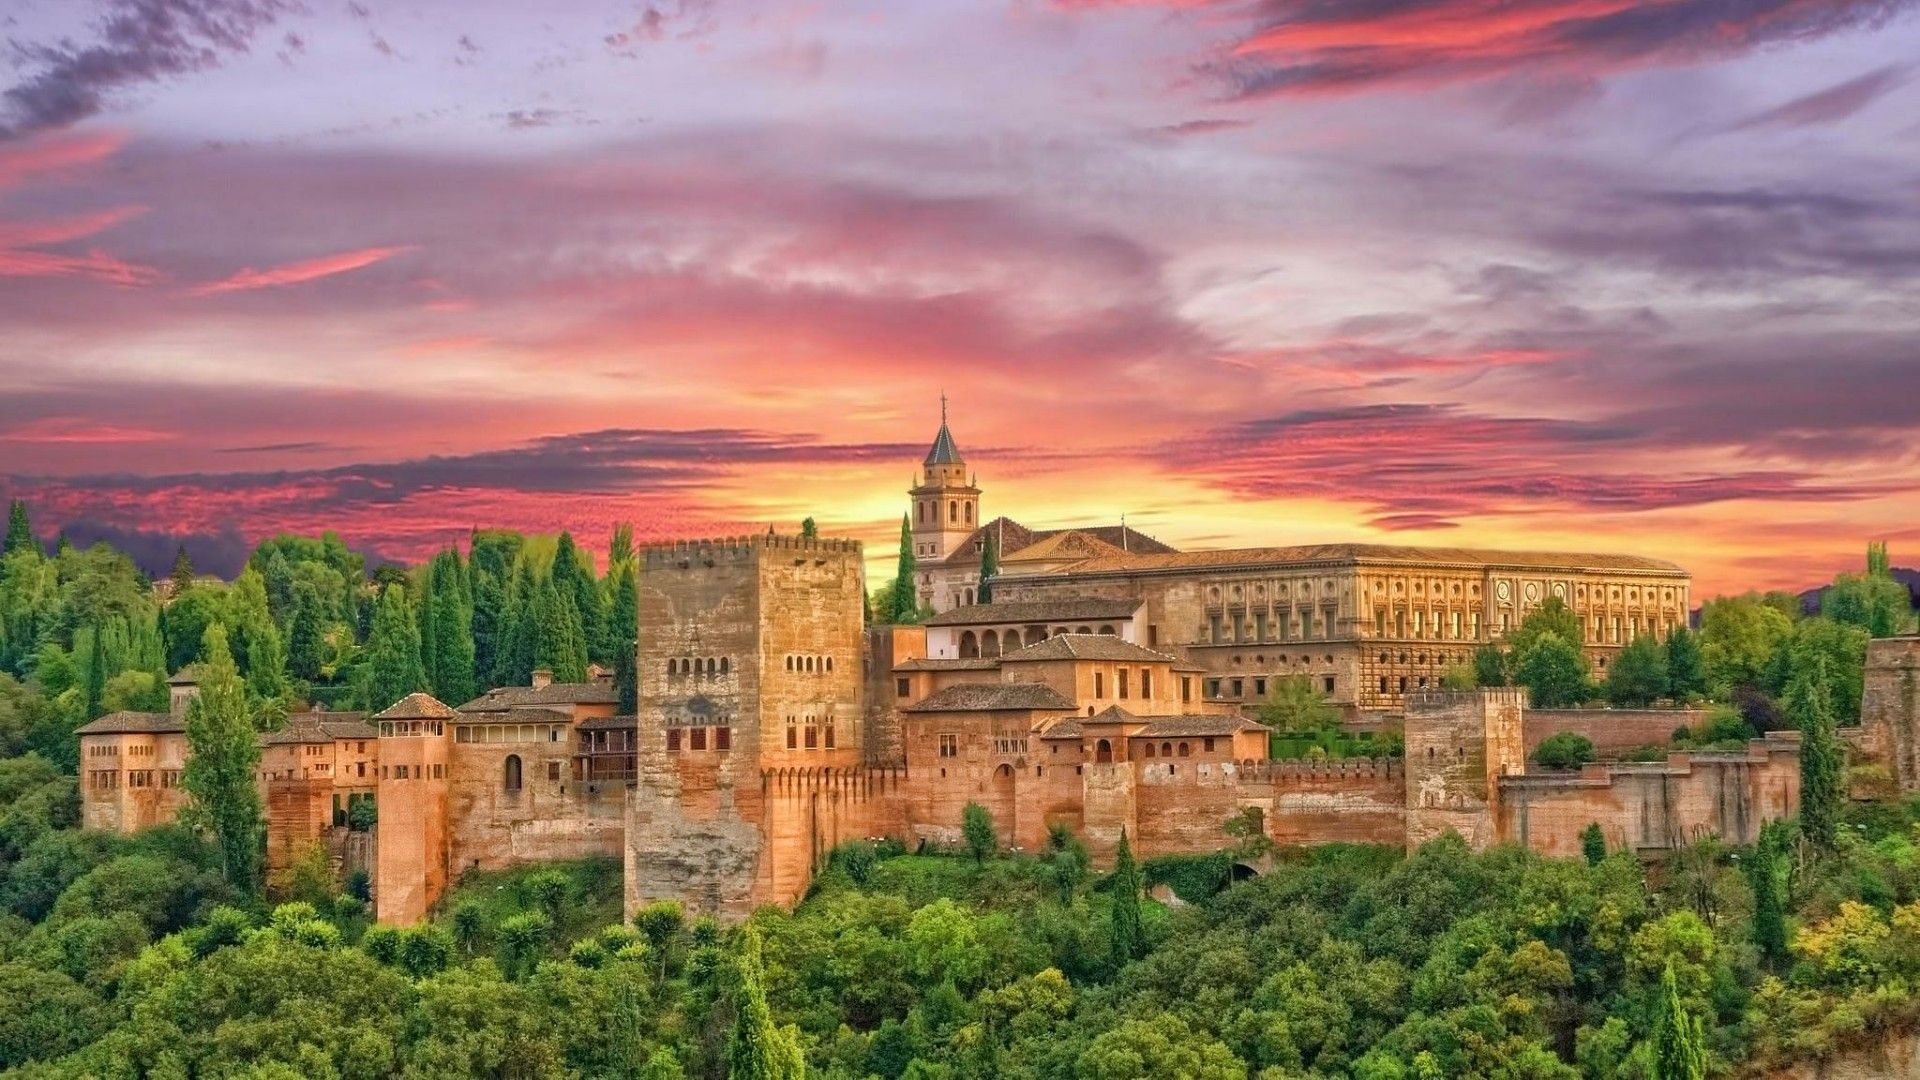
\includegraphics[width=\paperwidth,height=\paperheight,keepaspectratio]{images/granada.jpg}}
}

% Inicio del documento
\begin{document}

% Portada
\maketitle
\thispagestyle{empty}

\begin{center}
    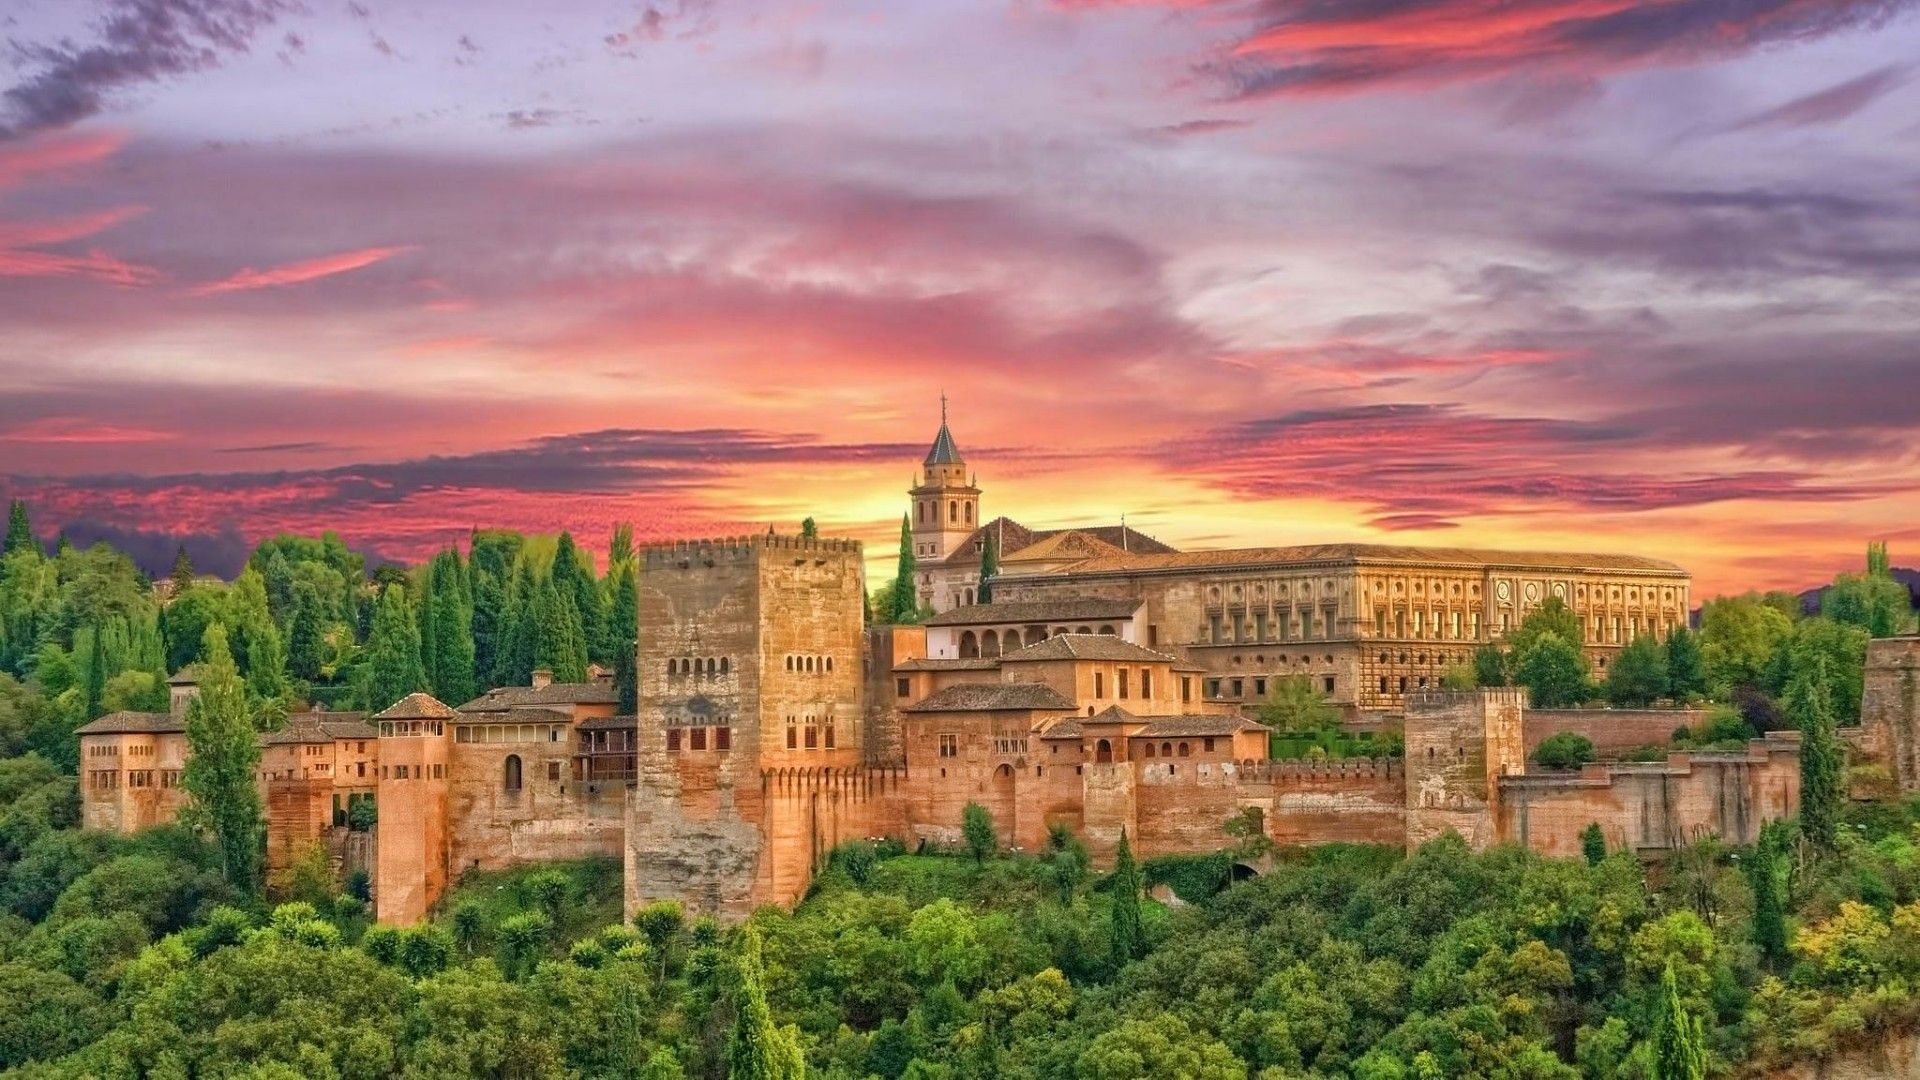
\includegraphics[width=\textwidth,height=0.4\textheight,keepaspectratio]{images/granada.jpg} \\ % Añade tu imagen de fondo
    \vfill
\end{center}

\newpage

% Índice
\tableofcontents
\thispagestyle{fancy}
\newpage

\textit{Nota: Los enunciados se encuentran en el libro.}

\section{Ejercicio 1}

\begin{itemize}
    \item Existencias iniciales = 80.000 \euro
    \item Deterioro = 5.000 \euro   
    \item Durante diciembre de 2020
    \begin{itemize}
        \item Compra 800 unidades a 12 \euro/unidad
        \item Descuento en factura de 400 \euro
        \item Gastos de transporte 500 \euro y se dejan a deber
    \end{itemize}
\end{itemize}

\begin{table}[H]
    \centering
    \begin{tabular}{|p{3cm}|p{6cm}|p{3cm}|}
    \hline
    \textbf{DEBE} & \textbf{Compra de Mercaderías} & \textbf{HABER} \\
    \hline
    \ecuacion{800 \times 12 - 400 + 500 = 9700}& \compraMercaderias & \\
    \hline
    \ecuacion{9700 \times 0,21 = 2037}& \IVAs & \\
    \hline
    & \bancos & \ecuacion{[9700 - 500] \times 1,21 = 11132}\\
    \hline
    & (410) Acreedores por prestación de servicios& \ecuacion{500 \times 1,21 = 605}\\
    \hline
    \end{tabular}
\end{table}

\begin{itemize}
    \item Devolvemos 100 unidades \footnote{Cálculo del nuevo precio(no lo pide):
    \begin{itemize}
        \item \ecuacion{100 \times 12 = 1200}
        \item Descuento para 100 unidades = \ecuacion{\frac{100  \times 400}{800} = 50}
        \item \ecuacion{1200 - 50 = 1150}
        \item Las que hay en el almacén = \ecuacion{800 - 100 = 700 \times 12 = 8400 - 350(\text{Descuento}) = 8050 + 500 (\text{transporte}) = 8550}
        \item \ecuacion{\frac{8550}{700} = 12,21 \text{ \euro/unidad}}
    \end{itemize}}
    \item Cargamos la cuenta 608 por \ecuacion{100 \times 12 - \text{decuento de 50} = 1150}
    \item Anticipo de proveedores

\end{itemize}
\begin{table}[H]
    \centering
    \begin{tabular}{|p{3cm}|p{6cm}|p{3cm}|}
    \hline
    \textbf{DEBE} & \textbf{Devolución de Mercaderías} & \textbf{HABER} \\
    \hline
    & \devCompr& 1150\\
    \hline
    & \IVAs& \ecuacion{1150 \times 0,21 = 241,5}\\
    \hline
    1150 & (407) Anticipo de proveedores & \\
    \hline
    241,5 & \IVAs & \\
    \hline
    \end{tabular}
\end{table}

\begin{itemize}
    \item Vende 900 unidades por 22.500 \euro
    \item Descuento en factura del 500 \euro
    \item A un cliente que había entregado un anticipo de 10.000 \euro
    \item En esta operación se incluye el anticipo
\end{itemize}

\begin{table}[H]
    \centering
    \begin{tabular}{|p{3cm}|p{6cm}|p{3cm}|}
    \hline
    \textbf{DEBE} & \textbf{Venta de Mercaderías} & \textbf{HABER} \\
    \hline
    \ecuacion{22500 - 500 - 10000 = 12000}& (430) Clientes  & \\
    \hline
    10.000 & (438) Anticipo a Clientes & \\
    \hline
    & \ventaMercaderias & 22.000\\
    \hline
    & \IVAr & \ecuacion{12000 \times 0,21 = 2520} \\
    \hline
    \end{tabular}
\end{table}

\begin{itemize}
    \item A \fec2020 la empresa tiene una existencias finales  = 60.000 \euro
    \item 2.000 \euro inservibles 
    \item Precio de venta del mercado 62.000 \euro
    \item costes de comercialización 3.000 \euro
    \item Valor neto realizable = 62.000 - 3.000 = 59.000 \euro
    \item \VC 60.000 - 2.000 = 58.000 \euro
    \item \valorrecuperable 59.000 \euro
    \item No hay deterioro, pero debemos de revertir el del incio que era de 5.000 \euro
\end{itemize}

\begin{table}[H]
    \centering
    \begin{tabular}{|p{3cm}|p{6cm}|p{3cm}|}
    \hline
    \textbf{DEBE} & \textbf{Operaciones relativas de la depreciación reversible e irreversible de Mercaderias a \fec2020} & \textbf{HABER} \\
    \hline
    80.000 & \varExist & \\
    \hline
    & \mercaderias & 80.000\\
    \hline
    58.000 & \mercaderias & \\
    \hline
    & \varExist & 58.000\\
    \hline
    & (390) Deterioro del valor de las mercaderías & \\
    \hline
    5.000 & (793) Reversión del deterioro de las mercaderias & \\
    \hline
    \end{tabular}
\end{table}

\section{Ejercicio 2}

\begin{itemize}
    \item Compra 500 unidades a 10,5 \euro/unidad
    \item Descuento por pronto pago incluido en factura de 250 \euro
    \item Precio de compra = \ecuacion{500 \times 10,5} = 5250 - 250 = 5000 \euro
    \item Gastos de transporte 500 \euro y se dejan a deber
\end{itemize}

\begin{table}[H]
    \centering
    \begin{tabular}{|p{3cm}|p{6cm}|p{3cm}|}
    \hline
    \textbf{DEBE} & \textbf{Compra de Mercaderías 02/03/2020} & \textbf{HABER} \\
    \hline
    5500 & \compraMercaderias & \\
    \hline
    \ecuacion{5500\times 0,21 = 1155}& \IVAs& \\
    \hline
    & (400) Proveedores & 6050\\
    \hline
    & (410) Acreedores por prestación de servicios & \ecuacion{500 \times 1,21 = 605}\\
    \hline
    \end{tabular}
\end{table}


\begin{itemize}
    \item El 23 de mayo se jubila el proveedor
    \item Descuento especial concedido de 425 \euro IVA no incluido
    \item Disminuye la deuda con él en esa cuantía
    \item Antes se produce una venta de 300 unidades por un importe de 4500 \euro
\end{itemize}

\begin{table}[H]
    \centering
    \begin{tabular}{|p{3cm}|p{6cm}|p{3cm}|}
    \hline
    \textbf{DEBE} & \textbf{Descuento especial concedido el 23/05/2020} & \textbf{HABER} \\
    \hline
    \ecuacion{4500\times1,21=5445}& (430) Clientes  & \\
    \hline
     & \ventaMercaderias & 4500\\
    \hline
    &\IVAr & 945\\
    \hline
    & (400) Proveedores & \\
    \hline
    & (778) Ingresos Excepcionales & 425\\
    \hline
    &\IVAs & 89,25\\
    \hline
    \end{tabular}
\end{table}

\begin{itemize}
    \item A \fec2020 la empresa tiene una pérdida irreversible 1000 \euro
    \item Precio de mercado = 17000 \euro
    \item Costes de comercialización 800 \euro
    \item Valor neto realizable = 17000 - 800 = 16200 \euro
    \item \VC = 17425 \euro
    \item \valorrecuperable = 17425 \euro
\end{itemize}
\begin{table}[H]
    \centering
    \begin{tabular}{|p{3cm}|p{6cm}|p{3cm}|}
    \hline
    \textbf{DEBE} & \textbf{Regularización de las Mercaderías a \fec2020} & \textbf{HABER} \\
    \hline
    15000& 610& \\
    \hline
    & 300 &15000 \\
    \hline
    & 610 &16000\\
    \hline
    16000 & 300& \\
    \hline
    \end{tabular}
\end{table}

\begin{itemize}
    \item Deterioro al inicio del ejercicio de 600 \euro
\end{itemize}

\begin{table}[H]
    \centering
    \begin{tabular}{|p{3cm}|p{6cm}|p{3cm}|}
    \hline
    \textbf{DEBE} & \textbf{Correcciones Valorativas} & \textbf{HABER} \\
    \hline
    600 & 390 & \\
    \hline
    & 793 & 600\\
    \hline
    \end{tabular}
\end{table}

\subsection{Ficha de almacén}
\textit{Usamos el Precio Medio Ponderado}

\begin{table}[H]
    \centering
    \begin{tabular}{|c|c|c|c|c|c|c|c|c|c|c|c}
        \hline
        \textbf{Categoría}  & \multicolumn{3}{c|}{\textbf{ENTRADAS}} & \multicolumn{3}{c|}{\textbf{SALIDAS}} & \multicolumn{3}{c|}{\textbf{EXISTENCIAS}} \\  \hline
        Existencias Iniciales & & & & & & & 1500 & 10 & 15000\\
        \hline
        Compra & 500 & 10,5 & 5250 & & & & 2000 & 10,25 & \\
        \hline
        Venta & & & & 300 & 10,25 & 4500&1700 &10,25 & 17425\\
        \hline
        Descuento & & (425)& & & & & 1700& 10& 17000\\
        \hline
        Pérdida& & (1000)& & & & & & & 16000\\
        \hline
        
    \end{tabular}    
\end{table}



\begin{itemize}
    \item En la compra el precio pasa a ser 10,25 \euro/unidad\footnote{\ecuacion{\text{Usando la fórmula de PMP} \rightarrow \frac{1500\times10+500\times10,5}{1500+500}=10,25}}.
    \item La venta se registra en la ficha de almacén por el valor que figura en la misma, no por lo que se vende.
    \item Podemos ver como hay valores que van entre paréntesis\footnote{Esto indica un valor negativo, es decir, pérdida, descuento, ...}.
\end{itemize}


\section{Resto de ejercicios}

Enlace a los ejericios hechos en otro formato: Pincha \href{https://github.com/ElblogdeIsmael/ElblogdeIsmael.github.io/blob/main/Asignaturas/Tercer%20A%C3%B1o/CF1/Practica/Tema2/EjerciciosPropuestos/FCCEE/Ejercicios_Profesor.pdf}{aquí}\footnote{Los que no están hechos de este documento o están en latex o no se han realizado por cuestiones de similitud a los realizados anteriormente}.


\end{document}